\subsubsection{\label{database} Database}

Dieses Paket\ref{fig:database_package}  kontrolliert alle Daten die in die Datenbank geschrieben werden.
Entweder sollen Daten in die Datenbank geschrieben werden, oder sie sollen ausgelesen werden. Die Antwort ist dementsprechend entweder leer, die gewünschten Daten, oder, im Fall von Unstimmigkeiten, eine Fehlermeldung.

Da jede Klasse auf dem Singleton Entwurfsmuster aufbaut wurden sämtliche darauf basierenden Parameter und Funktionen weggelassen.


\classWithoutPage{WorkflowData}
Diese Klasse ist die Schnittstelle für alle Klassen die auf den Datenbankeinträgen für Workflows arbeiten wollen. Sie erstellt für jeden Zugriff den passenden Datenbankbefehl und konvertiert die Ergebnisse in das gewünschte Format des Aufrufers.
Sie wirft bei fehlerhaften Werten eine entsprechende \textbf{MatFlowException}.

Diese Klasse, sowie alle anderen im Paket Database, ist nach dem Singleton Entwurfsmuster entworfen, da so Aufträge an die Datenbank so zentriert gesendet werden können.
\begin{figure}[h]
	\centering
	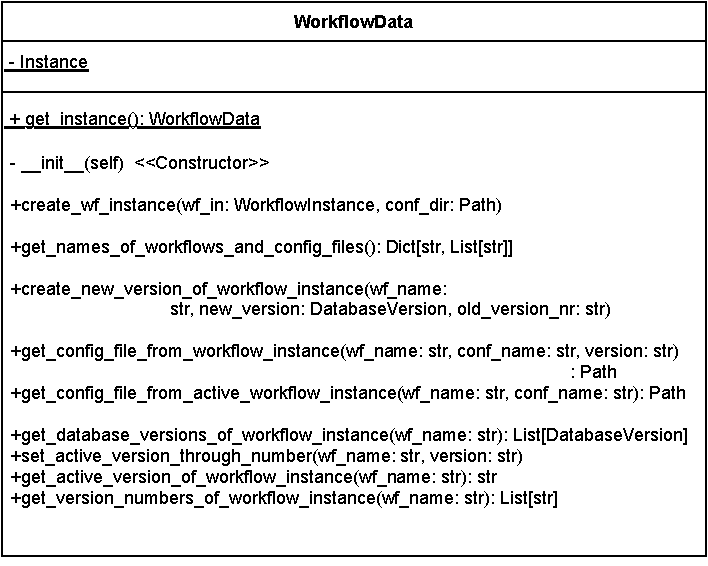
\includegraphics[width=0.7\textwidth]{res/Klassen/WorkflowData.pdf} 
	\caption{WorkflowData}
	\label{fig:workflowDataClass}
\end{figure}

\begin{methodenv}{Methods}

\method{create\textunderscore wf\textunderscore instance(wf\textunderscore in: WorkflowInstance, conf\textunderscore dir: Path):void}
Create a new instance of a workflow by using the dag-file of a Template, 
with the Version set to 1. 
Search confDirect for every .conf-file and add them into the Database.
Set this Version as active Version.

\smallPara{Parameters}
\begin{itemize}
	\item wf\textunderscore in
	new workflow
	\item conf\textunderscore dir
	path of folder with all .conf files for this workflow
\end{itemize}


\method{get\textunderscore names\textunderscore of\textunderscore workflows\textunderscore and\textunderscore config\textunderscore files():Dict[List[str]]}
Return all Workflow names and the names of their corresponding config files.
The returning value is a Dictionary with the workflow name as key, and lists of files as values

\method{create\textunderscore new\textunderscore version\textunderscore of\textunderscore workflow\textunderscore instance(wf\textunderscore name: str, new\textunderscore version: DatabaseVersion, old\textunderscore version\textunderscore nr: str):void}
Create a new Version of an existing Workflow with changed config Files.
Search which config Files changed and set those in the new Version.

\smallPara{Parameters}
\begin{itemize}
	\item \textbf{wf\textunderscore Name}
	name of the Workflow
	\item \textbf{new\textunderscore Verson}
	new Version
	\item \textbf{old\textunderscore version\textunderscore nr}
	identifier of Version the new one is based on
\end{itemize}

%new function
\method{get\textunderscore config\textunderscore file\textunderscore from\textunderscore workflow\textunderscore instance(wf\textunderscore name: str, conf\textunderscore name: str, version: str): Path}
Return single config file from a Workflow.

\smallPara{Parameters}
\begin{itemize}
	\item \textbf{wf\textunderscore name}
	name of the Workflow
	\item \textbf{conf\textunderscore name}
	name of conf file
	\item \textbf{version}
	version identifier
\end{itemize}
%new function end
%new function
\method{get\textunderscore config\textunderscore file\textunderscore from\textunderscore active\textunderscore workflow\textunderscore instance(self, wf\textunderscore name: str, conf\textunderscore name: str): Path}
Return single config file from active version of a Workflow.

\smallPara{Parameters}
\begin{itemize}
	\item \textbf{wf\textunderscore name}
	name of the Workflow
	\item \textbf{conf\textunderscore name}
	name of conf file
\end{itemize}
%new function end

\method{get\textunderscore database\textunderscore versions\textunderscore of\textunderscore workflow\textunderscore instance(wf\textunderscore name: str):List[DatabaseVersion]}
 Return all Versions of a Workflow Instance as DatabaseVersion Objects in a list.
 Asks the Database for the data and constructs every Object.
 
\smallPara{Parameters}
\begin{itemize}
	\item \textbf{wf\textunderscore name}
	name of the Workflow
\end{itemize}

\method{set\textunderscore active\textunderscore version\textunderscore through\textunderscore number(wf\textunderscore name: str, version: str):void}
Set the previous active Version as inactive and a new Version as active

\smallPara{Parameters}
\begin{itemize}
	\item \textbf{wf\textunderscore name}
	name of the Workflow
	\item \textbf{version}
	version to be set active
\end{itemize}

%new function
\method{get\textunderscore active\textunderscore version\textunderscore of\textunderscore workflow\textunderscore instance(self, wf\textunderscore name: str): str}
Return Version of Workflow set as active.

\smallPara{Parameters}
\begin{itemize}
	\item \textbf{wf\textunderscore name}
	name of the Workflow
\end{itemize}
%new function end

\method{get\textunderscore version\textunderscore numbers\textunderscore of\textunderscore workflow\textunderscore instance(wf\textunderscore name: str): List[str]}
Return a sortet list of Strings of all Versions of a Workflow.

\smallPara{Parameters}
\begin{itemize}
	\item \textbf{wf\textunderscore name}
	name of Workflow which versions should be listed
\end{itemize}

\end{methodenv}

%%%%%%%%%%%%%%%%%%%%%%%%%%%%%%%%%%%%%%%%%%%%%%%%%%%%%%%%%%%%%
%auskommentiert
\iffalse
\class{TemplateData}
Diese Klasse ist die Schnittstelle für alle Klassen die auf den Datenbankeinträgen für Workflow\\textunderscore Template arbeiten wollen. Sie erstellt für jeden Zugriff den passenden Datenbankbefehl und konvertiert die Ergebnisse in das gewünschte Format des Aufrufers.
Sie wirft bei fehlerhaften Werten eine entsprechende \textbf{MatFlowException}.

Diese Klasse, sowie alle anderen im Paket Database, ist nach dem Singleton Entwurfsmuster entworfen, da so Aufträge an die Datenbank so zentriert gesendet werden können.
\begin{figure}[h]
	\centering
	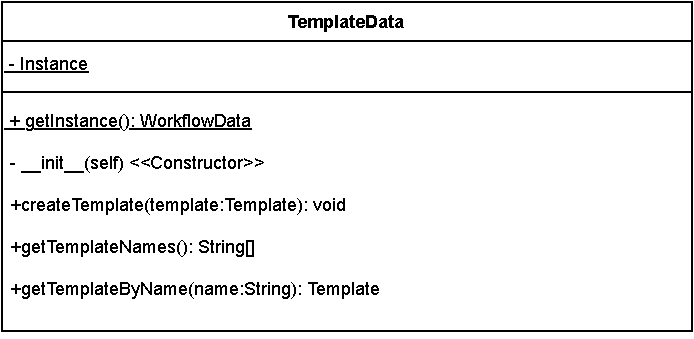
\includegraphics[width=0.7\textwidth]{res/Klassen/TemplateData.pdf} 
	\caption{WorkflowData}
	\label{fig:workflowDataClass}
\end{figure}

\begin{methodenv}{Methods}
	
\method{createTemplate(template:Template):void}
Read Values from template and convert them into a sql query.
Throw error if name already exists.

\smallPara{Parameters}
\begin{itemize}
	\item \textbf{template}
	Template object to convert
\end{itemize}

\method{getTemplateNames():str[]}
Return a list of all existing Template names.
List is empty when no Template exists.

\method{getTemplateByNames(name:str):Template}
Return Template that is asked for.
Throw error if Template doesn't exist.

\smallPara{Parameters}
\begin{itemize}
	\item \textbf{name}
	name/identifier of the wanted Template
\end{itemize}

\end{methodenv}
\fi
%%%%%%%%%%%%%%%%%%%%%%%%%%%%%%%%%%%%%%%%%%%%%%%%%%%%%%%%%%%%%%%%%%

\class{ServerData}
Diese Klasse ist die Schnittstelle für alle Klassen die auf den Datenbankeinträgen für Server arbeiten wollen. Sie erstellt für jeden Zugriff den passenden Datenbankbefehl und konvertiert die Ergebnisse in das gewünschte Format des Aufrufers.
Sie wirft bei fehlerhaften Werten eine entsprechende \textbf{MatFlowException}.

Diese Klasse, sowie alle anderen im Paket Database, ist nach dem Singleton Entwurfsmuster entworfen, da so Aufträge an die Datenbank so zentriert gesendet werden können.
\begin{figure}[h]
	\centering
	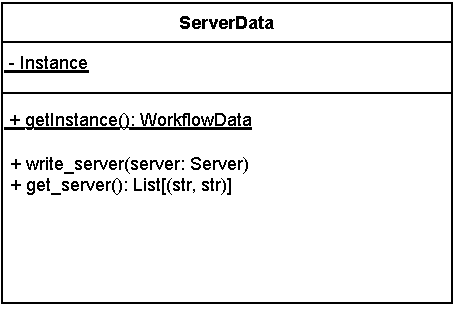
\includegraphics[width=0.7\textwidth]{res/Klassen/ServerData.pdf} 
	\caption{WorkflowData}
	\label{fig:workflowDataClass}
\end{figure}

\begin{methodenv}{Methods}
	
\method{write\textunderscore server(server: Server): void}
Write new Server into database.

\smallPara{Parameters}
\begin{itemize}
	\item \textbf{server} 
	Server object to get data from
\end{itemize}

\method{get\textunderscore server():List[(str, str)]} 
Get server in database.\\
NOTE: so far there should be only ever one server in the database, hence why no key is required.

\end{methodenv}
%%%%%%%%%%%%%%%%%%%%%%%%%%%%%%%%%%%%%%%%%%%%%%%%%%%%%%%%%%%%%%%%%%

\class{DatabaseTable}
DatabaseTable ist die einzige Klasse die direkt mit der Datenbank kommuniziert. Ihre Funktion ist hauptsächlich MySQL Befehle entgegennimmt, diese an die Datenbank weiterzugeben und die dadurch erhaltenen Antworten zurückgibt. Im Fall eines Fehlers, wie einem leeren Ergebnis oder eines ungültigen Befehls wird eine entsprechende \textbf{MatFlowException} geworfen.

Diese Klasse, sowie alle anderen im Paket Database, ist nach dem Singleton Entwurfsmuster entworfen, da so Aufträge an die Datenbank so zentriert gesendet werden können.
\begin{figure}[h]
	\centering
	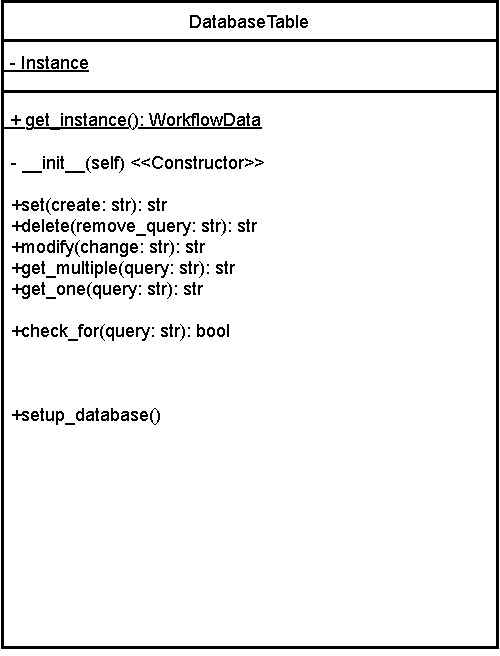
\includegraphics[width=0.7\textwidth]{res/Klassen/DatabaseTable.pdf} 
	\caption{WorkflowData}
	\label{fig:workflowDataClass}
\end{figure}

\begin{methodenv}{Methods}
	
	\method{set(create: str): str} Create new entry on Database. Try to execute create on Database and return value.
	
	\smallPara{Parameters}
	\begin{itemize}
		\item \textbf{create} 
		a sql query to create an entry
	\end{itemize}
	
	\method{delete(remove\textunderscore query: str): str} Delete an existing entry. Try to execute del on Database and return value.
	
	\smallPara{Parameters}
	\begin{itemize}
		\item \textbf{del} 
		a sql query to delete an entry
	\end{itemize}
	
	\method{modify(change: str): str} Modify an existing entry. Try to execute change on Database and return value.
	
	\smallPara{Parameters}
	\begin{itemize}
		\item \textbf{change} 
		a sql query to change values
	\end{itemize}

%new function
	\method{get\textunderscore multiple(query: str): str} 
	Search for multiple values in database.

	\smallPara{Parameters}
	\begin{itemize}
		\item \textbf{query} 
		sql query to get information
	\end{itemize}
%new function end
%new function
\method{get\textunderscore one(query: str): str}
Search for one(1)/first entry in database.

\smallPara{Parameters}
\begin{itemize}
	\item \textbf{query} 
	a sql query to get information
\end{itemize}
%new function end
%new function
\method{check\textunderscore for(self, query: str): bool}
Check if at least one(1) entry already exists for given SELECT-query.
True if at least one entry is found.

\smallPara{Parameters}
\begin{itemize}
	\item \textbf{query} 
	a sql query to get information
\end{itemize}
%new function end
%new function
\method{setup\textunderscore database(): void}
First setup of tables in the database.
Establish connection to Database with set parameters.
Read queries from external file and execute them.

Don't crash if tables already exist.
%new function end	
\end{methodenv}

\newpage